\subsection{Thread Spawner}

\begin{figure}[H]
	\centering
	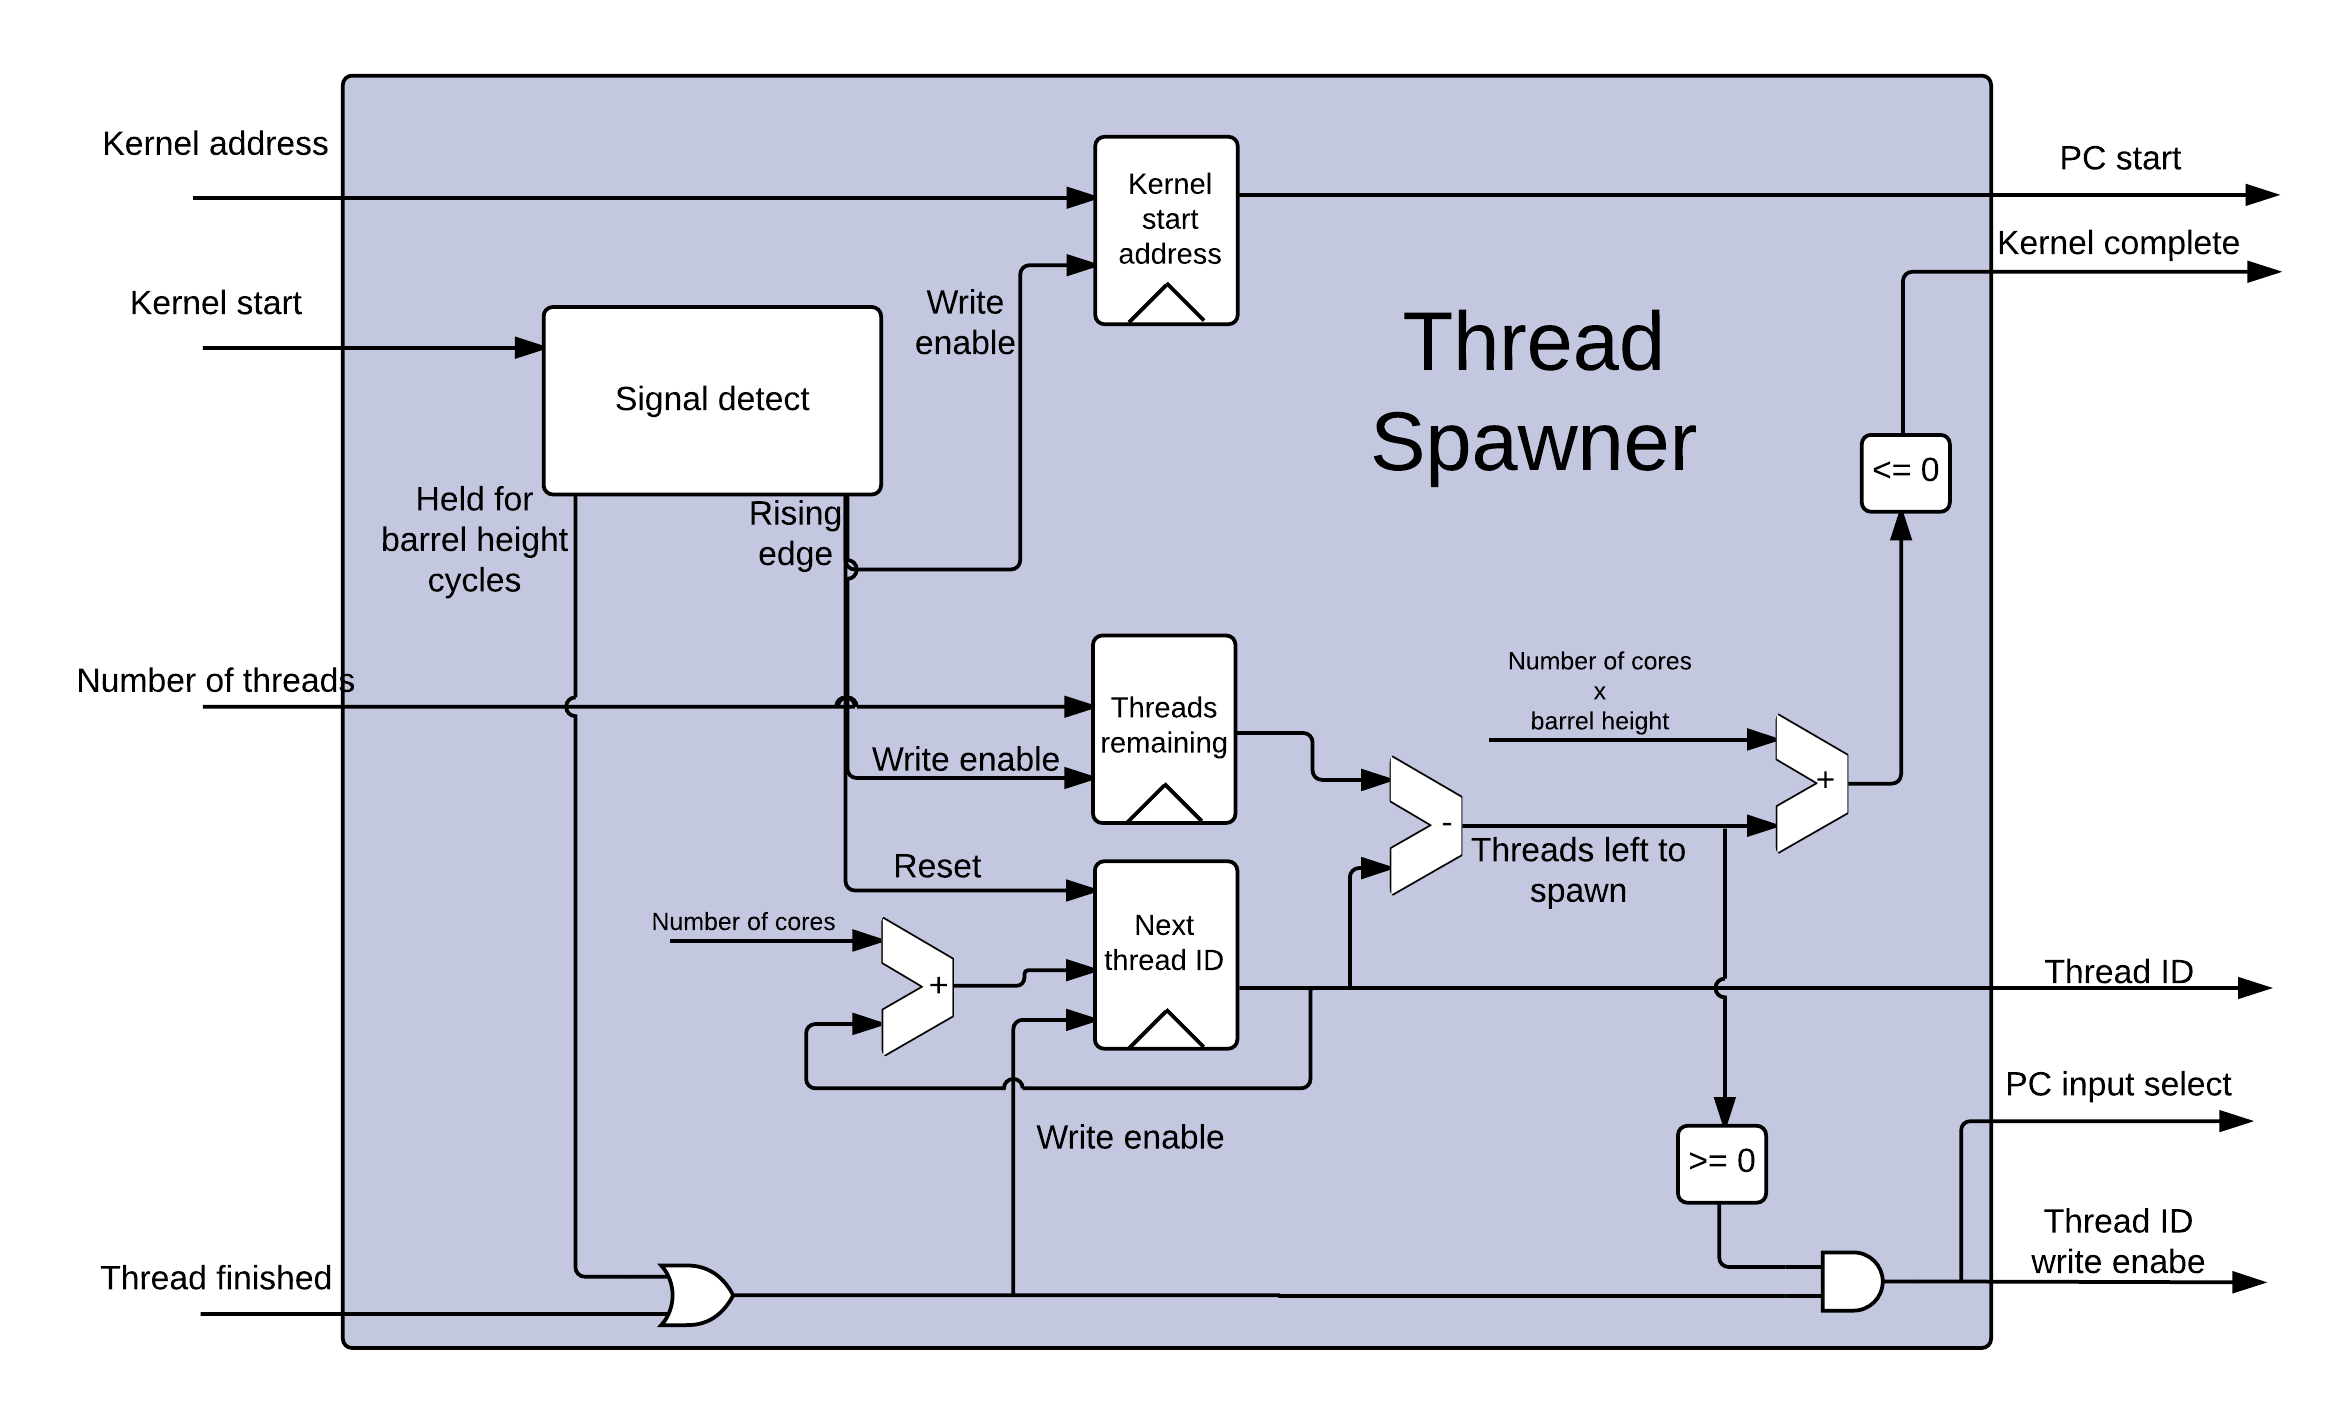
\includegraphics[width=\textwidth]{../gpu/diagrams/thread_spawner.png}
	\caption{Thread spawner and neighboring components}
	\label{fig:thread_spawner}
\end{figure}

The thread spawner is responsible for overseeing kernel execution.
It will spawn threads whenever necessary, handling thread setup and ensuring that the requested kernel is executed.
When all threads have finished executing, it will assert the kernel done signal, notifying the host program that computation has finished.

When a kernel invocation request is received, the thread spawner stores the provided base address of the kernel, the number of threads to spawn, and sets the next threadID register to zero.
Threads are spawned one warp at a time into the currently active barrel line.
Therefore, on kernel start the thread spawner will spawn threads until the warp drive has made an entire rotation.

When a thread finishes execution, the control unit will assert the 'finished' signal to the thread spawner.
If there are threads left to spawn, the currently active barrel row will be filled with a new warp of threads.

But what does the spawning of a warp of threads actually entail?
All threads need a unique threadID.
If the value of the next threadID register is 4, and we have 4 processor cores,
core zero will write 4 to its threadID register, core one 5, and so forth.
The next threadID register is then incremented by the warp size, increasing it from 4 to 8.

When a warp is spawned into barrel line zero, it signals that the first warp of a batch is about to be spawned.
The thread spawner uses this as a synchronization point to set the program counter to the base address of the current kernel.
The first instruction of the kernel start to trickle down the barrel lines shortly.

A new warp of threads has been spawned!
